%% Beginning of file 'sample631.tex'
%%
%% Modified 2021 March
%%
%% This is a sample manuscript marked up using the
%% AASTeX v6.31 LaTeX 2e macros.
%%
%% AASTeX is now based on Alexey Vikhlinin's emulateapj.cls 
%% (Copyright 2000-2015).  See the classfile for details.

%% AASTeX requires revtex4-1.cls and other external packages such as
%% latexsym, graphicx, amssymb, longtable, and epsf.  Note that as of 
%% Oct 2020, APS now uses revtex4.2e for its journals but remember that 
%% AASTeX v6+ still uses v4.1. All of these external packages should 
%% already be present in the modern TeX distributions but not always.
%% For example, revtex4.1 seems to be missing in the linux version of
%% TexLive 2020. One should be able to get all packages from www.ctan.org.
%% In particular, revtex v4.1 can be found at 
%% https://www.ctan.org/pkg/revtex4-1.

%% The first piece of markup in an AASTeX v6.x document is the \documentclass
%% command. LaTeX will ignore any data that comes before this command. The 
%% documentclass can take an optional argument to modify the output style.
%% The command below calls the preprint style which will produce a tightly 
%% typeset, one-column, single-spaced document.  It is the default and thus
%% does not need to be explicitly stated.
%%
%% using aastex version 6.3
\documentclass[twocolumn, linenumbers]{aastex631}

%% The default is a single spaced, 10 point font, single spaced article.
%% There are 5 other style options available via an optional argument. They
%% can be invoked like this:
%%
%% \documentclass[arguments]{aastex631}
%% 
%% where the layout options are:
%%
%%  twocolumn   : two text columns, 10 point font, single spaced article.
%%                This is the most compact and represent the final published
%%                derived PDF copy of the accepted manuscript from the publisher
%%  manuscript  : one text column, 12 point font, double spaced article.
%%  preprint    : one text column, 12 point font, single spaced article.  
%%  preprint2   : two text columns, 12 point font, single spaced article.
%%  modern      : a stylish, single text column, 12 point font, article with
%% 		  wider left and right margins. This uses the Daniel
%% 		  Foreman-Mackey and David Hogg design.
%%  RNAAS       : Supresses an abstract. Originally for RNAAS manuscripts 
%%                but now that abstracts are required this is obsolete for
%%                AAS Journals. Authors might need it for other reasons. DO NOT
%%                use \begin{abstract} and \end{abstract} with this style.
%%
%% Note that you can submit to the AAS Journals in any of these 6 styles.
%%
%% There are other optional arguments one can invoke to allow other stylistic
%% actions. The available options are:
%%
%%   astrosymb    : Loads Astrosymb font and define \astrocommands. 
%%   tighten      : Makes baselineskip slightly smaller, only works with 
%%                  the twocolumn substyle.
%%   times        : uses times font instead of the default
%%   linenumbers  : turn on lineno package.
%%   trackchanges : required to see the revision mark up and print its output
%%   longauthor   : Do not use the more compressed footnote style (default) for 
%%                  the author/collaboration/affiliations. Instead print all
%%                  affiliation information after each name. Creates a much 
%%                  longer author list but may be desirable for short 
%%                  author papers.
%% twocolappendix : make 2 column appendix.
%%   anonymous    : Do not show the authors, affiliations and acknowledgments 
%%                  for dual anonymous review.
%%
%% these can be used in any combination, e.g.
%%
%% \documentclass[twocolumn,linenumbers,trackchanges]{aastex631}
%%
%% AASTeX v6.* now includes \hyperref support. While we have built in specific
%% defaults into the classfile you can manually override them with the
%% \hypersetup command. For example,
%%
%% \hypersetup{linkcolor=red,citecolor=green,filecolor=cyan,urlcolor=magenta}
%%
%% will change the color of the internal links to red, the links to the
%% bibliography to green, the file links to cyan, and the external links to
%% magenta. Additional information on \hyperref options can be found here:
%% https://www.tug.org/applications/hyperref/manual.html#x1-40003
%%
%% Note that in v6.3 "bookmarks" has been changed to "true" in hyperref
%% to improve the accessibility of the compiled pdf file.
%%
%% If you want to create your own macros, you can do so
%% using \newcommand. Your macros should appear before
%% the \begin{document} command.
%%
\newcommand{\vdag}{(v)^\dagger}
\newcommand\aastex{AAS\TeX}
\newcommand\latex{La\TeX}

%% Reintroduced the \received and \accepted commands from AASTeX v5.2
%\received{March 1, 2021}
%\revised{April 1, 2021}
%\accepted{\today}

%% Command to document which AAS Journal the manuscript was submitted to.
%% Adds "Submitted to " the argument.
%\submitjournal{PSJ}

%% For manuscript that include authors in collaborations, AASTeX v6.31
%% builds on the \collaboration command to allow greater freedom to 
%% keep the traditional author+affiliation information but only show
%% subsets. The \collaboration command now must appear AFTER the group
%% of authors in the collaboration and it takes TWO arguments. The last
%% is still the collaboration identifier. The text given in this
%% argument is what will be shown in the manuscript. The first argument
%% is the number of author above the \collaboration command to show with
%% the collaboration text. If there are authors that are not part of any
%% collaboration the \nocollaboration command is used. This command takes
%% one argument which is also the number of authors above to show. A
%% dashed line is shown to indicate no collaboration. This example manuscript
%% shows how these commands work to display specific set of authors 
%% on the front page.
%%
%% For manuscript without any need to use \collaboration the 
%% \AuthorCollaborationLimit command from v6.2 can still be used to 
%% show a subset of authors.
%
%\AuthorCollaborationLimit=2
%
%% will only show Schwarz & Muench on the front page of the manuscript
%% (assuming the \collaboration and \nocollaboration commands are
%% commented out).
%%
%% Note that all of the author will be shown in the published article.
%% This feature is meant to be used prior to acceptance to make the
%% front end of a long author article more manageable. Please do not use
%% this functionality for manuscripts with less than 20 authors. Conversely,
%% please do use this when the number of authors exceeds 40.
%%
%% Use \allauthors at the manuscript end to show the full author list.
%% This command should only be used with \AuthorCollaborationLimit is used.

%% The following command can be used to set the latex table counters.  It
%% is needed in this document because it uses a mix of latex tabular and
%% AASTeX deluxetables.  In general it should not be needed.
%\setcounter{table}{1}

%%%%%%%%%%%%%%%%%%%%%%%%%%%%%%%%%%%%%%%%%%%%%%%%%%%%%%%%%%%%%%%%%%%%%%%%%%%%%%%%
%%
%% The following section outlines numerous optional output that
%% can be displayed in the front matter or as running meta-data.
%%
%% If you wish, you may supply running head information, although
%% this information may be modified by the editorial offices.
\shorttitle{ASPIRED toolkit}
\shortauthors{Lam et al.}
%%
%% You can add a light gray and diagonal water-mark to the first page 
%% with this command:
%% \watermark{text}
%% where "text", e.g. DRAFT, is the text to appear.  If the text is 
%% long you can control the water-mark size with:
%% \setwatermarkfontsize{dimension}
%% where dimension is any recognized LaTeX dimension, e.g. pt, in, etc.
%%
%%%%%%%%%%%%%%%%%%%%%%%%%%%%%%%%%%%%%%%%%%%%%%%%%%%%%%%%%%%%%%%%%%%%%%%%%%%%%%%%
\graphicspath{{./}{figures/}}
%% This is the end of the preamble.  Indicate the beginning of the
%% manuscript itself with \begin{document}.

\begin{document}

\title{Automated SpectroPhotometric Image REDuction (ASPIRED) -- \\ A \textsc{Python}-based spectral data reduction toolkit\\}



%% LaTeX will automatically break titles if they run longer than
%% one line. However, you may use \\ to force a line break if
%% you desire. In v6.31 you can include a footnote in the title.

%% A significant change from earlier AASTEX versions is in the structure for 
%% calling author and affiliations. The change was necessary to implement 
%% auto-indexing of affiliations which prior was a manual process that could 
%% easily be tedious in large author manuscripts.
%%
%% The \author command is the same as before except it now takes an optional
%% argument which is the 16 digit ORCID. The syntax is:
%% \author[xxxx-xxxx-xxxx-xxxx]{Author Name}
%%
%% This will hyperlink the author name to the author's ORCID page. Note that
%% during compilation, LaTeX will do some limited checking of the format of
%% the ID to make sure it is valid. If the "orcid-ID.png" image file is 
%% present or in the LaTeX pathway, the OrcID icon will appear next to
%% the authors name.
%%
%% Use \affiliation for affiliation information. The old \affil is now aliased
%% to \affiliation. AASTeX v6.31 will automatically index these in the header.
%% When a duplicate is found its index will be the same as its previous entry.
%%
%% Note that \altaffilmark and \altaffiltext have been removed and thus 
%% can not be used to document secondary affiliations. If they are used latex
%% will issue a specific error message and quit. Please use multiple 
%% \affiliation calls for to document more than one affiliation.
%%
%% The new \altaffiliation can be used to indicate some secondary information
%% such as fellowships. This command produces a non-numeric footnote that is
%% set away from the numeric \affiliation footnotes.  NOTE that if an
%% \altaffiliation command is used it must come BEFORE the \affiliation call,
%% right after the \author command, in order to place the footnotes in
%% the proper location.
%%
%% Use \email to set provide email addresses. Each \email will appear on its
%% own line so you can put multiple email address in one \email call. A new
%% \correspondingauthor command is available in V6.31 to identify the
%% corresponding author of the manuscript. It is the author's responsibility
%% to make sure this name is also in the author list.
%%
%% While authors can be grouped inside the same \author and \affiliation
%% commands it is better to have a single author for each. This allows for
%% one to exploit all the new benefits and should make book-keeping easier.
%%
%% If done correctly the peer review system will be able to
%% automatically put the author and affiliation information from the manuscript
%% and save the corresponding author the trouble of entering it by hand.

%\correspondingauthor{August Muench}
%\email{greg.schwarz@aas.org, gus.muench@aas.org}

\author[0000-0002-9347-2298]{Marco C. Lam}
\affiliation{School of Physics and Astronomy, Tel Aviv University, Tel Aviv 69978, Israel
}
\affiliation{Astrophysics Research Institute, Liverpool John Moores University, IC2, LSP, 146 Brownlow Hill, Liverpool L3 5RF, UK}
\affiliation{Astronomical Observatory, University of Warsaw, Al. Ujazdowskie 4, 00-478, Warszawa, Poland}

\author[0000-0003-3434-1922]{Robert J. Smith}
\affiliation{Astrophysics Research Institute, Liverpool John Moores University, IC2, LSP, 146 Brownlow Hill, Liverpool L3 5RF, UK}

\author[0000-0001-7090-4898]{Iair Arcavi}
\affiliation{School of Physics and Astronomy, Tel Aviv University, Tel Aviv 69978, Israel}
\affiliation{CIFAR Azrieli Global Scholars program, CIFAR, Toronto, Canada}

\author[0000-0001-8397-5759]{Iain A. Steele}
\affiliation{Astrophysics Research Institute, Liverpool John Moores University, IC2, LSP, 146 Brownlow Hill, Liverpool L3 5RF, UK}

\author[0000-0003-2780-7843]{Josh Veitch-Michaelis}
\affiliation{Astrophysics Research Institute, Liverpool John Moores University, IC2, LSP, 146 Brownlow Hill, Liverpool L3 5RF, UK}
\affiliation{Department of Physics and Wisconsin IceCube Particle Astrophysics Center, University of Wisconsin, Madison, WI 53706, USA}
\affiliation{ETH Z\"urich, Systems Group, Stampfenbachstrasse 114, 8092 Z\"urich, Switzerland}

\author[0000-0002-9658-6151]{Lukasz Wyrzykowski}
\affiliation{Astronomical Observatory, University of Warsaw, Al. Ujazdowskie 4, 00-478, Warszawa, Poland}


%% Note that the \and command from previous versions of AASTeX is now
%% depreciated in this version as it is no longer necessary. AASTeX 
%% automatically takes care of all commas and "and"s between authors names.

%% AASTeX 6.31 has the new \collaboration and \nocollaboration commands to
%% provide the collaboration status of a group of authors. These commands 
%% can be used either before or after the list of corresponding authors. The
%% argument for \collaboration is the collaboration identifier. Authors are
%% encouraged to surround collaboration identifiers with ()s. The 
%% \nocollaboration command takes no argument and exists to indicate that
%% the nearby authors are not part of surrounding collaborations.

%% Mark off the abstract in the ``abstract'' environment. 
\begin{abstract}

We provide a suite of publicly available spectral data reduction software to facilitate
rapid scientific products from time-domain observations. The Automated SpectroPhotometric
REDuction (\textsc{ASPIRED}) toolkit is aimed to be as general as possible with high flexibility
such that it can work with different instruments. The default settings support typical
low-resolution long-slit spectrometer configurations, whilst it also offers a flexible set of
functions for users to refine and tailor-make automated pipelines to an instrument's
individual characteristics. Automation can provide immediate data reduction to allow adaptive
observing strategies, which is particularly important in Time Domain Astronomy. \textsc{ASPIRED} is
entirely \textsc{Python}-based and is independent of \textsc{iraf}.


\end{abstract}

%% Keywords should appear after the \end{abstract} command. 
%% The AAS Journals now uses Unified Astronomy Thesaurus concepts:
%% https://astrothesaurus.org
%% You will be asked to selected these concepts during the submission process
%% but this old "keyword" functionality is maintained in case authors want
%% to include these concepts in their preprints.
\keywords{(fill in)}

%% From the front matter, we move on to the body of the paper.
%% Sections are demarcated by \section and \subsection, respectively.
%% Observe the use of the LaTeX \label
%% command after the \subsection to give a symbolic KEY to the
%% subsection for cross-referencing in a \ref command.
%% You can use LaTeX's \ref and \label commands to keep track of
%% cross-references to sections, equations, tables, and figures.
%% That way, if you change the order of any elements, LaTeX will
%% automatically renumber them.
%%
%% We recommend that authors also use the natbib \citep
%% and \citet commands to identify citations.  The citations are
%% tied to the reference list via symbolic KEYs. The KEY corresponds
%% to the KEY in the \bibitem in the reference list below. 


\section{Introduction}
With major global investments in multi-wavelength and multi-messenger surveys, time-domain
astronomy is entering a golden age. In order to maximally exploit discoveries from these
facilities, rapid spectroscopic follow-up observations of transient objects~(e.g.,\ supernovae,
gravitational-wave optical counterparts etc.) is needed to provide crucial {\em astrophysical} 
interpretations. Part of the former OPTICON\footnote{\url{https://www.astro-opticon.org}; now the
OPTICON-RadioNet Pilot \url{https://www.orp-h2020.eu}} project coordinates the operation of a
network of largely self-funded European robotic and conventional telescopes, coordinating
common science goals and providing the tools to deliver science-ready photometric and
spectroscopic data in near real-time. The goal is to facilitate automated or interactive
decision making, allowing ``on-the-fly'' modification of observing strategies and rapid
triggering of other facilities. As part of the network's activity, a software development work package was
commissioned under the working title of Automated SpectroPhotometric REDuction (\textsc{ASPIRED})
toolkit, coordinated on Github\footnote{\url{https://github.com/cylammarco/ASPIRED}}.

The ``industrial standard'' of spectral and image reduction is of no doubt the
\textsc{iraf} software~\citep{1986SPIE..627..733T, 1993ASPC...52..173T}. It has powered many
reduction engines in the past and present. However, unfortunately, the software has reached
the end-of-support state where there will no longer be any official support to the software
, and it relies entirely on community support\footnote{\url{https://iraf-community.github.io}}.

In this generation of user-side Astronomy data handling and processing, as well as the emphasis in
computing courses for scientists, \textsc{Python} is among the most popular languages due to
its ease to use with a shallow learning curve, readable syntax and simple way to ``glue''
different pieces of software together. Its flexibility to serve as a scripting and an
object-oriented language makes it useful in many use cases: demonstrating with visual tools
with little overhead, prototyping, web-serving, and it can be compiled if wanted. This broad range of
functionality and high-level usage make it relatively inefficient. However, \textsc{Python}
is an excellent choice of language to build wrappers over highly efficient and well-established
codes. In fact, some of the most used packages,
\textsc{scipy}~\citep{2020SciPy-NMeth} and \textsc{numpy}~\citep{2020NumPy-Array},
are written in \textsc{Fortran} and \textsc{C} respectively. Multi-threading and multi-processing
are also possible with built-in and other third-party packages, e.g.\ \textsc{mpi4py}~\citep{DALCIN20111124}. 

Various efforts are being made to develop software for current and next-generation 
spectral data reduction. For example, \textsc{PypeIt}~\citep{pypeit:zenodo, pypeit:joss_pub}
is designed for tailor-made reductions of various instruments, \textsc{PyReduce}~\citep{2021A&A...646A..32P}
is designed for optimal Echelle spectral reduction (but does not handle sky subtraction);
in the \textsc{Astropy} `Universe'~\citep{astropy:2013, astropy:2018}, \textsc{specreduce}
is likely to be the next-generation user-focused data reduction package, but it is far from
the stage of deployment at the time of writing. \textsc{pyDIS} has all the essential
ingredients for reducing spectra but has been out of maintenance since 2016, and \textsc{specutils}
handles spectral analysis and manipulation but not the reduction itself.

In \textsc{ASPIRED}, we have a different vision in how and what should be abstracted from the
users. Instead of providing a ready-to-go `black box' suited for a specific instrument
or observations made in particular conditions, we provide a toolkit that is as general
as possible for users to have a set of high-level data reduction building blocks to
process the data in the ways most appropriate to their instruments and observations.
This shifts more of the work and maintenance to the user-end, but it will allow rapid
modification of the data reduction workflow if there are any changes in the instrumental
configuration, for example, a detector is refitted, and the detector plane is shifted and
rotated by a few pixels. \textsc{ASPIRED} also aims to provide a set of functions that requires
coding skills that students  should have attained from university-level of Observational
Astrophysics course.

We use the SPRAT family as our `first-light' instruments for development~\citep{2014SPIE.9147E..8HP},
but we aim to allow high-level tools for users to build and fine-tune their pipelines to support
a wide range of configurations~\citep{2020arXiv201203505L, marco_2021_4463569}. As of the time of
writing, we have successfully used \textsc{ASPIRED} to reduce data from the William Herschel Telescope
\textit{Intermediate-dispersion Spectrograph and Imaging System}
\footnote{\url{https://www.ing.iac.es/astronomy/instruments/isis}}~(WHT/ISIS), Las Cumbres
Observatory FLOYDS~\citep[LCO/FLOYDS]{2013PASP..125.1031B}, Gemini Observatory
\textit{Gemini Multi-Object Spectrographs} long slit
mode~\citep[Gemini/GMOS-LS]{2004PASP..116..425H}, Gran Telescopio Canarias \textit{Optical
System for Imaging and low-Intermediate-Resolution Integrated
Spectroscopy}~\citep[GTC/OSIRIS]{2000SPIE.4008..623C}, and Telescopio Nazionale Galileo
\textit{Device Optimised for the LOw
RESolution\footnote{\url{http://www.tng.iac.es/instruments/lrs}}}~(TNG/DOLORES); all of
these are currently still unofficial sets of reduction procedures. The examples of these deployments can be
found at \url{https://github.com/cylammarco/aspired-example}.

This paper is organised as follows: Section \textsection2 covers the software's development and
organisation. Then, we go through the details of the spectral reduction
procedures in Section \textsection3. In the last section, we provide various links
for references and instructions for installation.

This article is not intended to serve as an API document, nor as a review of the
various methods concerning spectral extraction. Only the high-level
descriptions and the scientific and mathematical technicalities that are
important to the data reduction processes are discussed here.

\section{Development and Structure of \textsc{ASPIRED}}

One of the development goals of \textsc{ASPIRED} is to design a piece of software that is as
modular and portable as possible. We rely on as few external dependencies as possible.
The ones we do use are those that would require a substantial programming effort to reproduce and have a
proven track record of reliability and/or plan to remain maintained in the
foreseeable future. The explicit top-level dependencies are --
\textsc{astroscrappy}~\citep{curtis_mccully_2018_1482019, 2001PASP..113.1420V}
\textsc{astropy}~\citep{astropy:2013, astropy:2018},
\textsc{ccdproc}~\citep{matt_craig_2017_1069648},
\textsc{numpy}~\citep{2020NumPy-Array}
\textsc{plotly}~\citep{plotly},
\textsc{scipy}~\citep{2020SciPy-NMeth}
\textsc{spectres}~\citep{2017arXiv170505165C}, and
\textsc{statsmodels}~\citep{seabold2010statsmodels}. 

We host our source code on Github, which provides version control and other
utilities to facilitate the development. It uses \textsc{git}\footnote{\url{https://git-scm.com}},
issue and bug tracking, high-level project management, automation with \textsc{Github Actions}
upon each \texttt{commit} for:

\begin{enumerate}
    \item Continuous Integration~(CI) to install the software in \textsc{Linux}, \textsc{Mac} and \textsc{Windows} system, and then perform unit tests with \textsc{pytest}~\citep{pytest6.2},
    \item generating test coverage report with \textsc{Coveralls}\footnote{\url{https://coveralls.io/github/cylammarco/ASPIRED}} which identifies lines in the script that are missed from the tests,
    \item Continuous Deployment~(CD) through \textsc{PyPI}\footnote{\url{https://pypi.org/project/aspired}} that allows immediate availability of the latest numbered version,
    \item dependency version tracking with \textsc{Dependabot}\footnote{\url{https://dependabot.com}}, and
    \item generating API documentation powered by \textsc{Sphinx}\footnote{\url{https://www.sphinx-doc.org/en/master}} hosted on Read the Docs\footnote{\url{https://aspired.readthedocs.io/en/latest}}.
\end{enumerate}

The initial
work package divided the project broadly into three high-level independent
components:

\subsubsection*{Graphical User Interface\\(not in active development)}
In the beginning, we commissioned a prototype of the graphical user
interface\footnote{\url{https://github.com/cylammarco/gASPIRED}}
\textsc{Electron}\footnote{\url{https://www.electronjs.org}}, which wraps on top of
\textsc{ASPIRED} without needing to adapt the code. This is
possible for a few reasons: first, \textsc{Python} is an interpreter, it can execute
in run time - it is straightforward to run itself as a server to handle the response from 
\textsc{Electron}; second, there are many plotting libraries available, and there is
not a unified API standard for creating a figure. It is difficult to maintain
multiple plotting libraries to optimise certain plots for diagnostics and
visualisations; \textsc{plotly}\footnote{\url{https://plotly.com}} has a good balance
generating interactive and static plots, so it is chosen as our plotting engine; third,
there is a \textsc{JavaScript} version of
\textsc{SAOImageDS9}\footnote{\url{https://sites.google.com/cfa.harvard.edu/saoimageds9}}
that allows rapid and easy interactive image manipulation in a familiar
fashion~\citep{eric_mandel_2021_596052}. Given how \textsc{Electron} and
\textsc{JS9} work like a web service, this prototype also shows that it can 
be deployed as an online tool. Such high-level of interactivity is, however, no longer
in active development and currently only serves as a technology demonstrator of its capability.

\subsubsection*{Wavelength Calibration\\(not part of this work)}
The wavelength calibration module is powered by the RANSAC Assisted Spectral CALibration
~(\textsc{RASCAL}, \citealt{2020zndo...4117517V, 2020ASPC..527..627V}, Veitch-Michaelis
\& Lam in prep.), a software package developed in conjunction but independently of \textsc{ASPIRED}.
It is improved on the work by \citet{2018ApOpt..57.6876S}, which searches only for
\textit{plausible} sets of arc lines that follow good linear approximations to the
system. \textsc{RASCAL} considers the top $N$ sets simultaneously. For each peak~(pixel),
the most common best-fit atlas line~(wavelength) is chosen from the top candidate
sets. This acts like a piece-wise linear fit and allows us to extract most of
the correct matches from both the red and blue ends of the spectrum. RANdom
SAmple Consensus~\citep[RANSAC,][]{fischler_bolles_1981} is used to robustly
fit a higher-order polynomial model to the candidate correspondences. The user
is only required to supply a list of calibration lines~(pixels), a
list of peaks~(wavelengths), and some knowledge~(e.g.\ dispersion resolution) of
the system to initialise a most appropriate and efficient calibrator object for
fitting the pixel-to-wavelength solution.

\subsubsection*{Data Reduction and Other Calibrations\\(this work)}
This is the core of the \textsc{ASPIRED}, which mainly handles the spectral
extraction and calibration processes. The software is organised into
3 main parts -- \texttt{image\_reduction}, \texttt{spectral\_reduction},
and \texttt{spectrum1D}. The first two are the ``overlords'' that handle
all the dependent classes and functions to orchestrate the operations.
The third is a data structure that stores the metadata and the extracted
data. The FITS file I/O handling is also handled by \texttt{spectrum1D}.


\subsection{Data Reduction Modules}

\subsubsection{\texttt{image\_reduction}}
This module allows combining, subtracting and dividing of light,
dark, bias and flat frames. The FITS header of the first light frame provided
is copied over, while the headers from the other frames are not stored -- only
the file paths are stored as meta-data. The image reduction meta-data
are appended to the end of the FITS header. Depending on the convention
adopted by the observatories, the FITS file is defaulted to contain an empty \texttt{PrimaryHDU}
with the process data stored in the first \texttt{ImageHDU} extension as
recommended in the FITS Standard 
document\footnote{\url{https://fits.gsfc.nasa.gov/fits_documentation.html}},
or it can be stored directly in the \texttt{PrimaryHDU} as most users tend
to opt for. Many forms of interactive and static images can be exported,
powered by the \textsc{Plotly} image renderer.

\textsc{ASPIRED} intends to provide basic image reduction methods, sufficient for simple
optical systems, which are the primary targets of \textsc{ASPIRED}. For
example, a long slit spectrograph with a rectilinear 2D spectrum illuminated
on the detector plane, i.e. the dispersion and spatial directions are perfectly
perpendicular to each other across the entire detector plane. It is usually
not immediately suitable for complex systems that have multiple non-parallel
spectra illuminated on the detector plane. In the FLOYDS reduction example,
we demonstrate how two non-parallel, highly curved spectra in a single
2D spectral image can be reduced and extracted by applying a mask to the
data.

\subsubsection{\texttt{spectral\_reduction}}
This is a large module that covers both 1D and 2D operations. In 2D, it
provides image rectification, spectral tracing and spectral extraction.
In 1D, it can perform wavelength calibration, flux calibration, atmospheric
extinction correction and Telluric absorption correction. Diagnostic images
can be exported at each step of operation, including the wavelength calibration
that wraps around \textsc{RASCAL} and uses their native plotting capability.
Outputs can be in FITS or ASCII files, e.g.\ CSV, where possible. See the next
section for the mathematical and scientific descriptions of the various methods.

\subsubsection{\texttt{spectrum1D}}
This module provides a uniform format to store the metadata
and the extracted data throughout the entire spectral extraction process.
Data storage of observational data is almost exclusively done with FITS files,
but they are not human readable. In view of that, \textsc{ASPIRED} provides I/O handling
of both FITS and ASCII-type files. All the higher-level functions are wrappers on
top of a \texttt{spectrum1D} object.

\section{Spectral Reduction}
In the highest-level terms, spectral reduction procedures after image
reduction include: (1) identifying the spectrum/a, (2) tracing the
spectrum/a, (3) correcting for image distortion, (4) extracting the
spectrum/a, (5) performing wavelength calibration of the science target and a
standard star, (6) computing the sensitivity curve using the standard
observations, (7) performing atmospheric extinction correction,
and finally (8) removing Telluric absorption. We omit a few common
processes which we believe should be considered as part of the
post-extraction processes or spectral analysis and manipulation.
There are many sophisticated software packages with good and long track records
to handle these processes post hoc. For example, sky glow subtraction
with \textsc{Skycorr}~\citep{2014A&A...567A..25N}, or Telluric
absorption removal \textbf{wihtout} supplementary calibration data with
\textsc{MoleFit}~\citep{2015A&A...576A..77S, 2015A&A...576A..78K}.
The following describes the technical details of the eight steps,
where we use the following convention: the spectral image is dispersed
on the detector plane such that the left side (small pixel number) corresponds to
the blue part of the spectrum and the right side (large pixel number) to the red part.

\subsection{Spectral Identification and Tracing}
\label{sec:tracing}
Conventionally, to obtain the position of a spectrum (i.e.\ trace), the centre of
a spectrum in the dispersion direction is first identified, then a choice
algorithm will scan across the spectral image to identify the spectral position
over the entire dispersion direction. Instead, in \textsc{ASPIRED}, the \texttt{ap\_trace()}
function works by dividing the 2D spectrum into sub-spectra, and then each part
is summed along the spectral direction before cross-correlating with the adjacent
sub-spectra. This way, both the shift and the scaling of the spectrum/a along the
spectral direction can be found simultaneously. The middle of the
2D spectrum is used as the zero point of the procedure. Here is a
detailed description of the algorithm:
\begin{enumerate}
    \item
        The input 2D spectrum is divided into \texttt{nwindow}
        sub-spectra.
    \item
        Each sub-spectrum is summed along the spectral direction
        in order to improve the signal(s) of the spectrum/a along
        the spatial direction – we call this a spatial spectrum.
    \item
        Each spatial spectrum is upscaled by a factor of
        \texttt{resample\_factor} to allow for sub-pixel correlation
        precision. This utilises the \texttt{scipy.signal.resample()}
        function to fit the spatial profile with a spline.
    \item
        The i-th spatial spectrum is then cross-correlated to the i+1-th
        spatial spectrum. The shift and scale where the maximum
        occurs within the tolerance limit, \texttt{tol} is then stored.
    \item
        The shifts relative to the central sub-spectrum are used to
        fit for a polynomial solution that defines the position of
        the trace.
    \item
        While the spatial spectra are cross-correlated, they
        are aligned and stacked for peak finding and Gaussian fitting
        towards the end of the iteration. Peak finding is performed with
        \texttt{scipy.signal.find\_peaks()} and returns the list of
        peaks sorted by their prominence. Only centroiding has to be
        accurate at this stage, so a Gaussian function is sufficient.
        The standard deviation of the Gaussian is only served as a
        first guess of the profile when performing optimal extraction;
        it would not be used in the case of top-hat extraction (see
        section \textsection3.3).
\end{enumerate}

This procedure is illustrated in Fig.~\ref{fig:trace}. Manually
supplying a trace is possible with the \texttt{add\_trace()}
function. This is particularly useful for faint and/or confused
sources that are beyond the capability of automated tracing. For
example, if there is a faint transient source on top of a galaxy,
a manual offset may be needed for extraction if the host is
dominating the flux to a level that forced extraction is necessary.
Otherwise, we recommend extracting the two (or more) most significant
peaks for validation; the number needed depends on
the environment and the morphology of the galaxy.

\begin{figure}
    \centering
    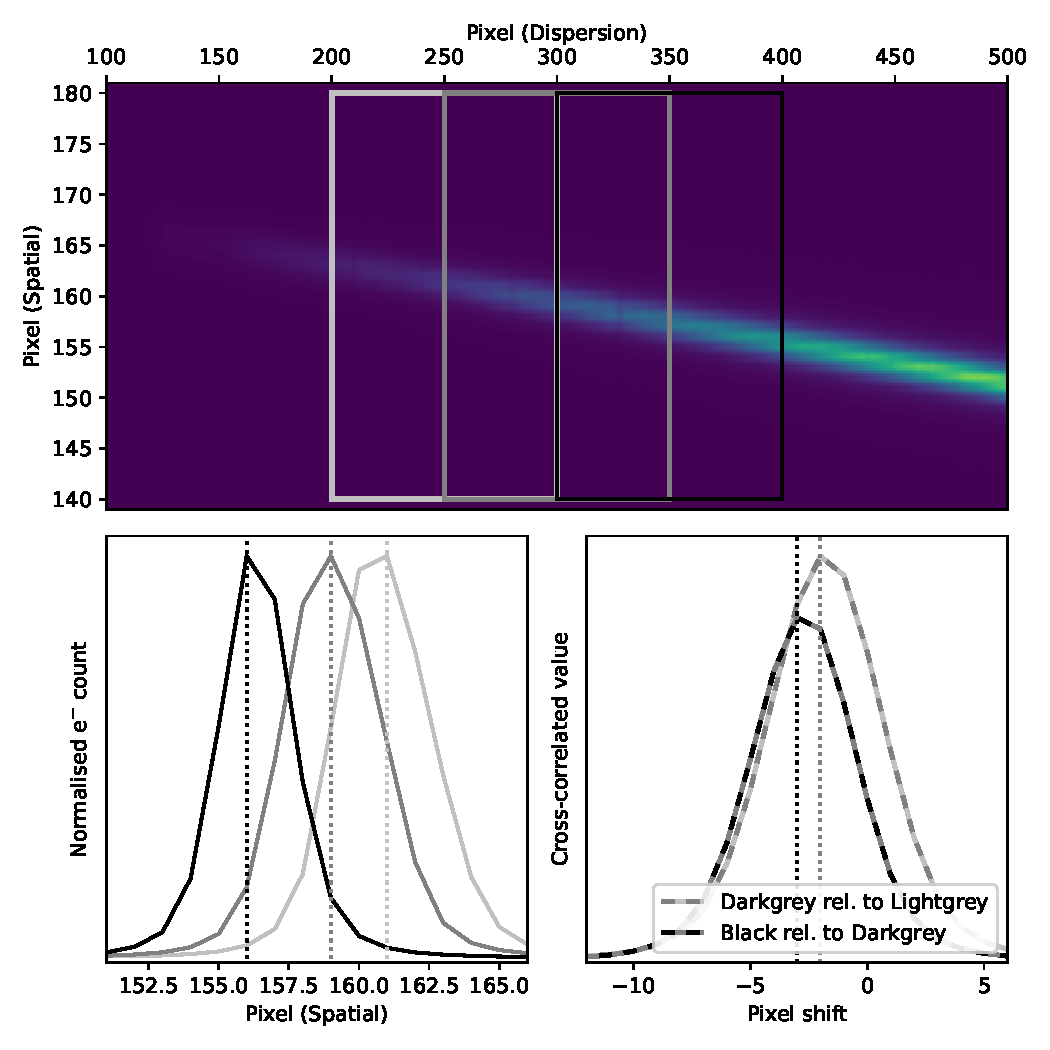
\includegraphics[width=\columnwidth]{fig_01_tracing.pdf}
    \caption{Top: A LT/SPRAT spectrum is rotated to illustrate how
    cross-correlation is used to find the shift between neighbouring
    sub-spectra. The orange, green and blue boxes are three example
    sub-spectra. Bottom left: the three sub-spectra are summed in
    the dispersion direction to generate the three profiles that are
    cross-correlated to compute the shift. Bottom right: the
    cross-correlated function for the green sub-spectrum relative
    to the orange sub-spectrum (plotted in green), and the one
    for the blue sub-spectrum relative to the green sub-spectrum
    (plotted in blue).}
    \label{fig:trace}
\end{figure}


\subsection{Image Rectification}
In most cases, a spectrum on the detector plane is not only tilted,
but it is also sufficiently distorted that the extraction has to be
performed along a curve in order to perform sky subtraction properly.
While this does not cause any complication in the tracing, the
spatial and dispersion directions are no longer aligned with the x-y
axes of the detector plane. \textsc{PyReduce} can optimally extract
such highly distorted spectra, but the lack of sky subtraction using
the ``wings'' in the sky region beyond the line-spread-profile has
limited the usage in a typical single-frame extraction without an
accompanying sky observation at an identical slit position.
Alternatively to extracting along a curve, the 2D image can be
rectified based on the spectral trace and sky emission or arc lines
before extraction, so that the latter is performed on a spectrum~(nearly)
perfectly aligned with the detector x-y axes. Using the arc frame for
this process will deliver a more reliable rectification function.

The rectification in the spatial direction depends \textbf{only}
on the trace. Each column of pixels gets (scaled and) shifted by
resampling to align with the centre of the spectrum. This will
usually leave us with a spectrum tilted or curved in the dispersion
direction. Therefore, the same procedure for tracing the spectra is
applied in the spatial direction to find the best fit polynomial
solution for shifting (and scaling) in the dispersion direction for
the second step of the rectification process (See Fig.~\ref{fig:rectify}).

\begin{figure}
    \centering
    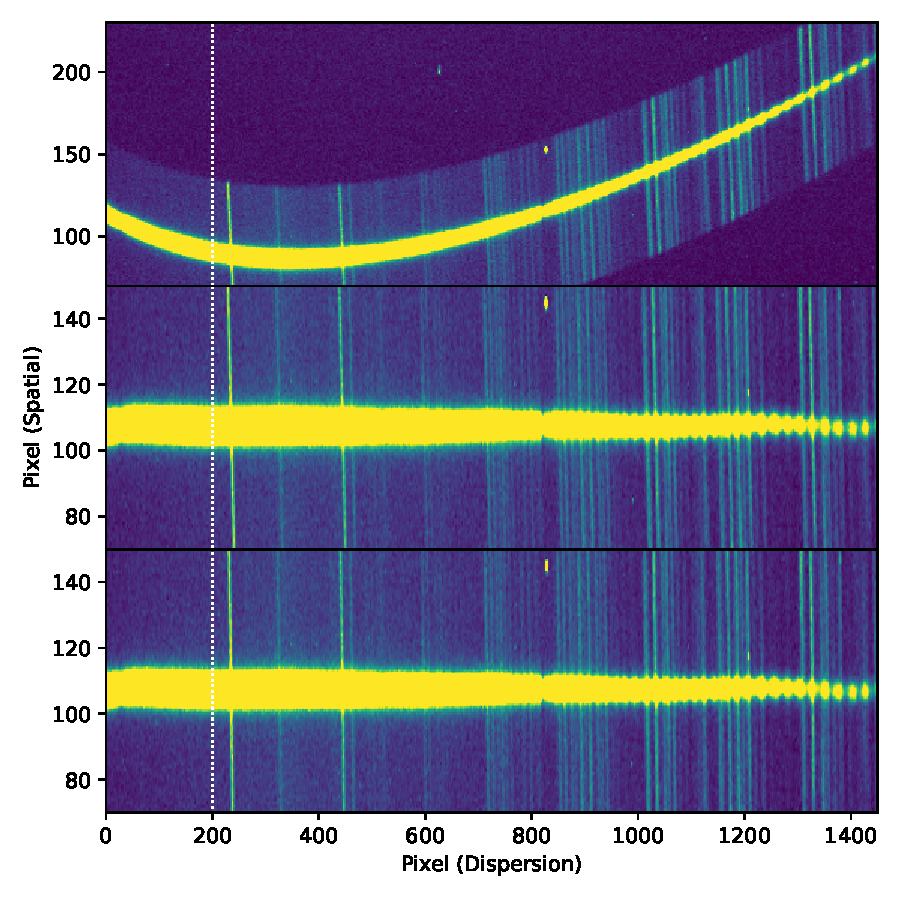
\includegraphics[width=\columnwidth]{fig_02_rectification.pdf}
    \caption{A 2D spectrum from LCO/FLOYDS is used to
    demonstrate the rectification procedure. The dotted white line
    is aligned in the spatial direction to serve as a visual guide.
    Top: The trimmed image of a FLOYDS spectrum. Middle: The 2D
    spectrum is resampled in the spatial direction based on the
    polynomial function of the trace. Bottom: The 2D spectrum is
    resampled in the dispersion direction. The shifts and scales
    are found by cross-correlating the sub-spectra divided in the
    spatial direction. This is perpendicular to the tracing process.}
    \label{fig:rectify}
\end{figure}

At the time of writing, this process is only possible if there is
one trace. If more than one trace is found/provided, only the first
one will get processed. The resampling is performed with
\texttt{scipy.ndimage.zoom} which interpolates with a spline (the
electron count is not always perfectly conserved, but the difference
is negligible). It is possible to supply a set of pre-computed polynomials to perform
the rectification, which can significantly speed up the data reduction
process of a stable optical system.

\subsection{Spectral Extraction}
\label{sec:extract}
There are a few commonly used extraction methods; some work for
all kinds of spectral images, some only work with specific
observing strategies (e.g. the flat-relative optimal
extraction;~\citealt{2014A&A...561A..59Z}). The standard textbook
method is commonly called the \textit{top-hat} extraction or the
\textit{normal} extraction. It simply sums the electron counts over
a given size of the aperture, and is robust and easy to use. However,
this method does not deliver the maximal signal-to-noise ratio~(SNR)
from the available data. Various optimal extraction algorithms
can increase the SNR. This works by down-weighting the wings of the
spectral profile where almost all the photons are coming from the sky
rather than the source~(see Fig.~\ref{fig:extinction}). An optimal
extraction can boost the SNR, particularly for background-limited
sources, which are the case in most observations~(see
Fig.~\ref{fig:extraction_compared}). The extracted spectra and their
associated uncertainties and sky background counts can be plotted
for inspection. The residual image can also be exported for diagnostics.

\begin{figure}
    \centering
    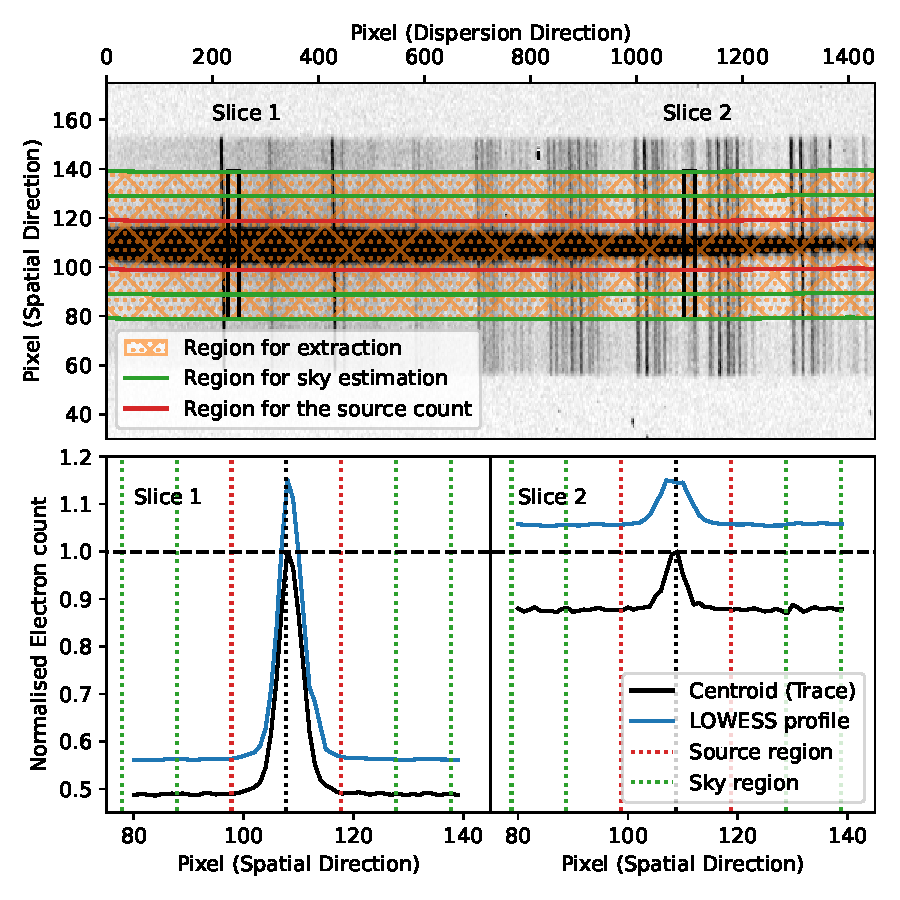
\includegraphics[width=\columnwidth]{fig_03_extraction_profile.pdf}
    \caption{The same spectrum as in Figure~\ref{fig:rectify} but the
    2D spectral image is slightly rotated to have the sky lines
    aligned with the spatial direction with the y-axis.
    Top: The regions used for source and sky extractions are marked
    by the red and green lines and arrows. The light shade of orange
    hash marks denotes the entire region that is used for spectral extraction.
    The two boxes show the two columns of pixels fitted with
    profiles in the bottom half of the figure (the boxes are inflated
    for clarity). Bottom: The electron counts across the two slices,
    The vertical black dashed line is the centroid~(trace) of the spectrum,
    the two red dashed lines mark the regions of the source and the
    pairs of green dashed lines on each side of the centroid are
    showing the regions used for sky extractions, respectively. The
    black line is the measured spectral profile (data), the blue
    line is the fitted LOWESS line-spread-function (model), offset for
    clarity.}
    \label{fig:extraction}
\end{figure}

\subsubsection*{Tophat/Normal Extraction}
The top-hat extraction does not weigh the pixels for extraction,
so every pixel has an equal contribution to the source count. Thus,
it is very robust in getting the total electron count across
a slice of pixels. The sky background count can be extracted
from the regions outside the extraction aperture to be
subtracted from the spectrum.

\subsubsection*{Horne-86 Optimal Extraction}
\citet[hereafter H86]{1986PASP...98..609H} is the golden standard
of optimal extraction of spectra from modern electronic detectors.
We follow the H86 recipe except for the profile modelling,
where we provide three options: The first is a fixed Gaussian
profile, the second uses LOcally Weighted Scatterplot
Smoothing~\citep[LOWESS]{doi:10.1080/01621459.1979.10481038}
regression to fit for a polynomial, and the third accepts
a manually supplied profile.

The default option is to use the LOWESS fit because it is the
least sensitive to noise, cosmic ray contamination and detector
artefacts. It is also flexible enough to allow a good fit for
the profile of a resolved galaxy. This may, however, be less
accurate for extracting a faint spectrum when the image is
dominated by background noise. In such a case, the Gaussian
profile is recommended as the profile is constructed from fitting
the line-spread function from the total stack of all the
sub-spectra~(as described in Sec.~\ref{sec:tracing}). The quality
of a valid profile should be as good as an extraction
performed with the top-hat extraction method.

\subsubsection*{Marsh-89 Optimal Extraction}
\citet[hereafter M89]{1989PASP..101.1032M} improves on the H86
algorithm by fitting the change in the shape and centroid of the
profile from one end of the spectrum to the other. It is very
suited for extracting a highly tilted spectrum where the tilting
direction is aligned with only \textbf{one} direction in the $x-$
or the $y$-axis of the detector. Here we adapt Ian Crossfield's set of public
\textsc{Python 2} code for Astronomy\footnote{\url{https://people.ucsc.edu/~ianc/python/}}$^,$\footnote{\url{https://crossfield.ku.edu/python/}}
to \textsc{Python 3}.

\begin{figure}
    \centering
    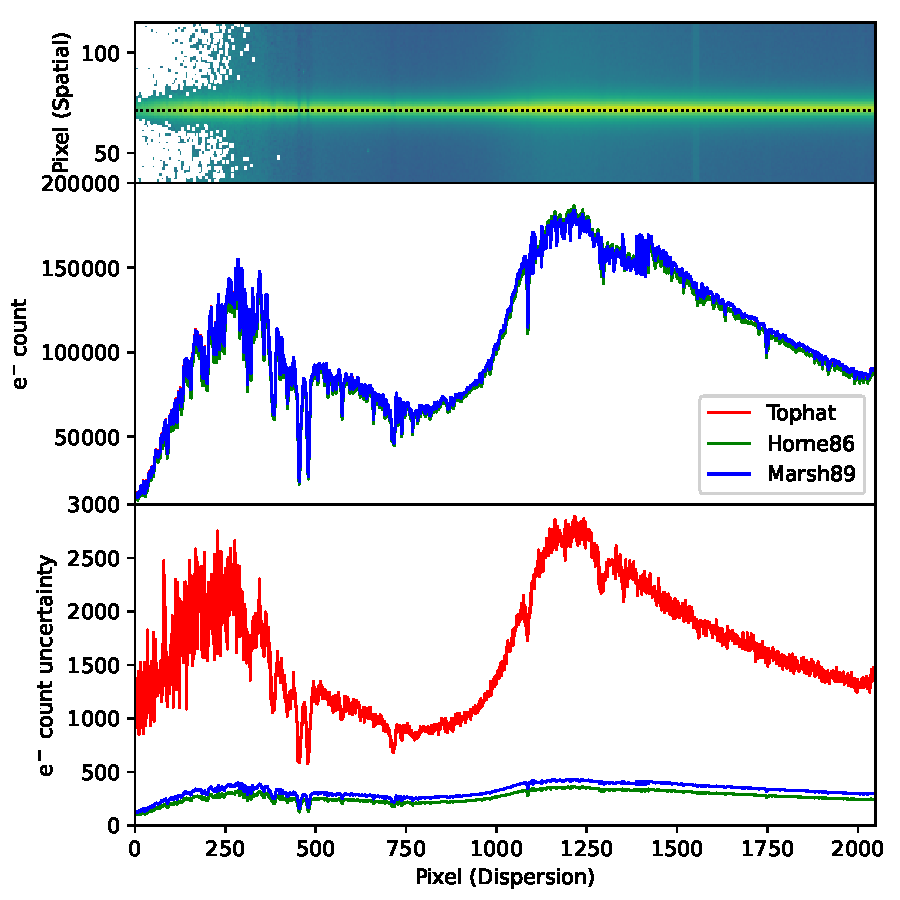
\includegraphics[width=\columnwidth]{fig_04_extraction_compared.pdf}
    \caption{Top: An LT/SPRAT spectrum of a featureless ultra-cool white dwarf PSO J1801+625~\citep{2020MNRAS.493.6001L}.
    Middle: The extracted spectra in electron counts using the three extraction methods
    are very similar. Bottom: The uncertainties with the three extraction methods
    in units of electron counts. The
    top-hat method is clearly noisier than the two optimal methods at the faint ends of the spectrum.}
    \label{fig:extraction_compared}
\end{figure}

\subsection{Wavelength Calibration}
The wavelength calibration is powered by \textsc{RASCAL}, which
is a concurrent development to this work. All the public
functions from \textsc{RASCAL} are available in \textsc{ASPIRED}
so users can have fine control over the calibration. The
diagnostic plots are the set provided by \textsc{RASCAL}.
They include the spectrum of the arc lamp where the traces
on the science and standard frames are, which also shows where
the peaks are detected; the peak-line pairs and the constrained
space where the Hough-pairs are
selected~(see \citealt{2020ASPC..527..627V}); and a plot showing
the fitting solution and its quality~(Fig.~\ref{fig:wavecal}).

The polynomial coefficients for the calibration can be supplied
directly, which would be useful for stable instruments in which
the variations in the dispersion are negligible.

\begin{figure}
    \centering
    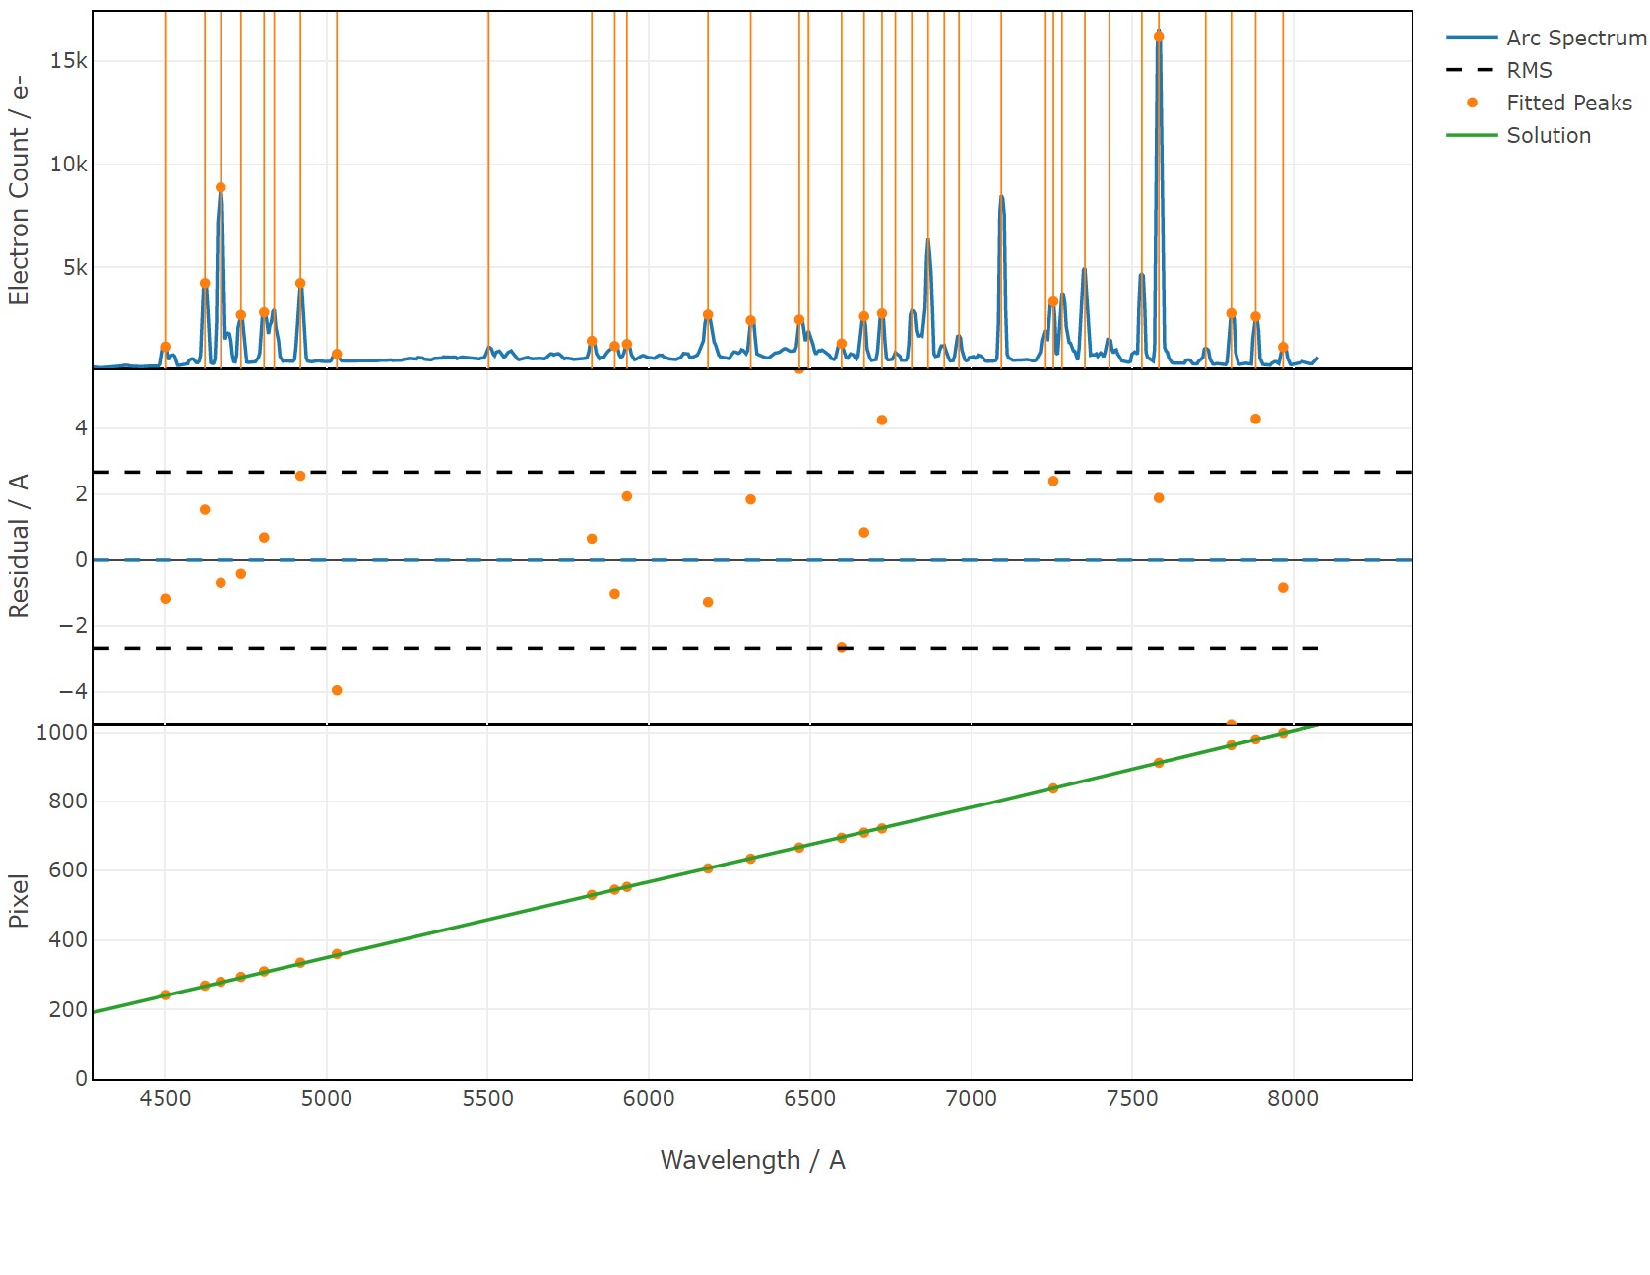
\includegraphics[width=\columnwidth]{fig_05_wavelength_calibration_diagnostics.pdf}
    \caption{The wavelength calibration diagnostic plots from RASCAL.
    Top: the arc is plotted in blue, the fitted peaks are marked by
    the orange dots. Middle: The residual plot shows the difference
    between the fitted peaks and the true wavelengths. Bottom: The
    pixel-wavelength function (green) is overplotted with the fitted
    peaks (orange).}
    \label{fig:wavecal}
\end{figure}

\subsection{Flux Calibration}
When a standard spectrum is wavelength calibrated, it can be
compared against literature values to obtain the sensitivity
function of the detector. All the standard stars available in
\textsc{iraf}\footnote{\url{https://github.com/iraf-community/iraf/tree/main/noao/lib/onedstds}}
and on the ESO webpage -- \textit{Optical and UV Spectrophotometric
Standard Stars}\footnote{\url{https://www.eso.org/sci/observing/tools/standards/spectra.html}}
are available on \textsc{ASPIRED}. See Appendix ~\ref{appendix:standards} for
the complete listing of the standard stars and the respective data
source. The calibration can be done in either AB magnitude or
flux density~(per unit wavelength). The two should give similar
results, but the response functions found would not be equivalent
because fitting to magnitudes is in logarithmic space and smoothing~(see
below) will have a different effect compared to flux fitting.

\subsubsection*{Smoothing}
A Savitzky-Golay smoothing
filter\footnote{\url{https://docs.scipy.org/doc/scipy/reference/generated/scipy.signal.savgol_filter.html}}~\citep[hereafter, SG-filter]{1964AnaCh..36.1627S}
can be applied to the data before computing the sensitivity curve.
This function works by fitting low-order polynomials to localised
subsets of the data to suppress noise in the data at each point
interval. It is similar to the commonly used median boxcar filter,
but uses more weighted information to better
retain information while removing noise. This can be
used independently or with continuum fitting (see below), which
uses a LOWESS filter. By default, the SG-filter removes only
significant noise~(e.g.\ those from unsubtracted cosmic rays).

\subsubsection*{Continuum Fitting}
By default, the continuum of the standard spectrum is found for
deriving the sensitivity curve. This process is used after the
smoothing procedure~(if performed). The continuum is found by
fitting the standard spectrum with a LOWESS function as described in
Sec.~\ref{sec:extract}. This can remove any outlying random noise
as well as the absorption lines when computing the sensitivity. Users
are reminded to be cautious with this procedure as the removal of the
absorption features in computing the sensitivity function can
significantly affect the flux calibration near the absorption features.

\subsubsection*{Sensitivity Curve}
The sensitivity curve is computed by dividing the observed standard
spectrum by the literature one and then interpolating the result using a
spline or a polynomial function~(Fig.~\ref{fig:fluxcal}. This can be
done with or without any pre-smoothing and/or continuum fitting. Users
can also manually supply a sensitivity function as a callable function
that accepts a wavelength value and returns the $\log$ of the sensitivity
value at that wavelength. The sensitivity function does not carry the
concept of units; it can be magnitude, flux, or any other appropriate
unit (if supplied manually).

\begin{figure}
    \centering
    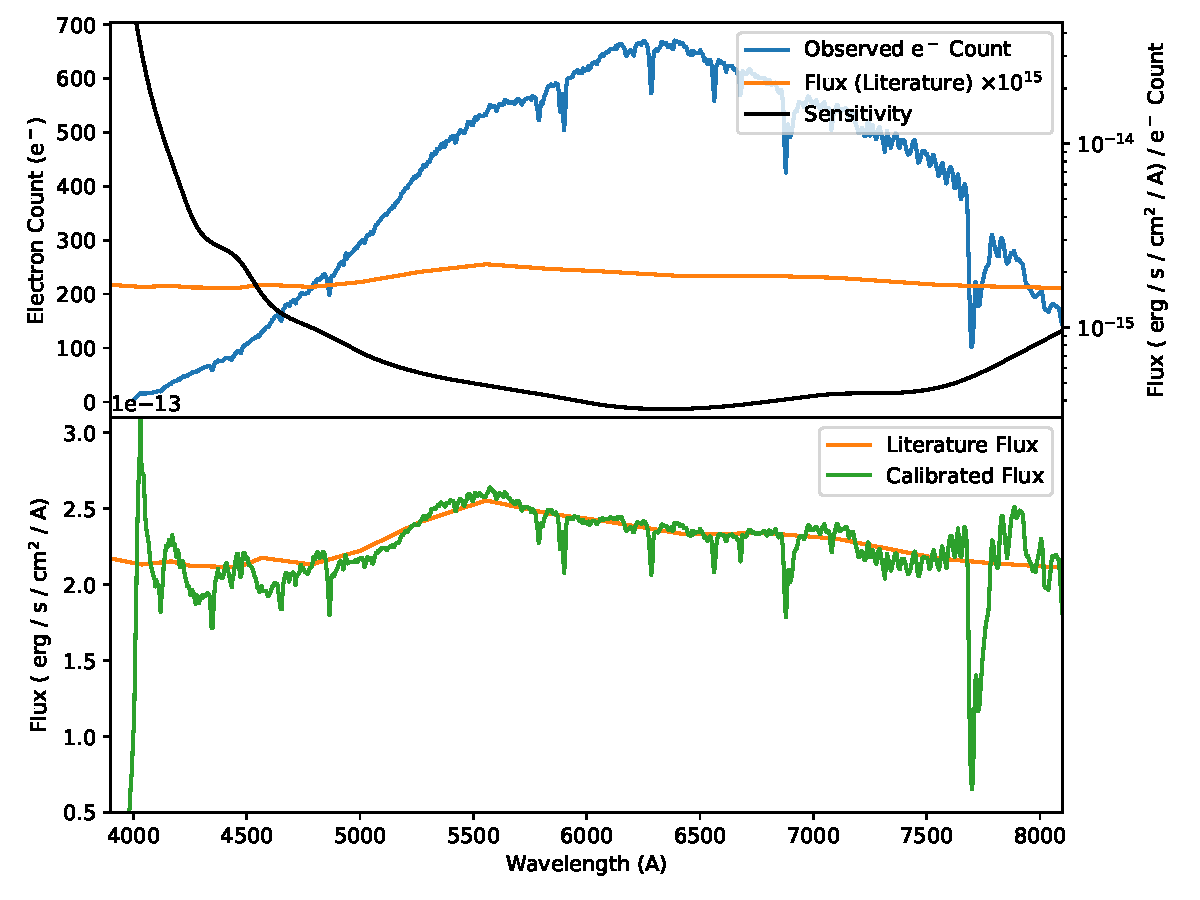
\includegraphics[width=\columnwidth]{fig_06_flux_calibration_diagnostics.pdf}
    \caption{Top: The extracted standard spectrum in electron counts
    (blue), the literature spectrum in units of flux density (multiplied
    by $10^{17}$; colour), and the sensitivity function (y-axis on the right; black).
    Bottom: The literature spectrum (same as the one above) is plotted
    in orange, and the calibrated observed spectrum is plotted in green.}
    \label{fig:fluxcal}
\end{figure}

\subsection{Atmospheric Extinction Correction}
\textsc{ASPIRED} currently has four built-in atmospheric extinction curves:

\begin{enumerate}
    \item Roque de los Muchachos Observatory~(2420\,m)\footnote{\url{http://www.ing.iac.es/astronomy/observing/manuals/ps/tech\_notes/tn031.pdf}}
    \item Mauna Kea Observatories~\citep[4205\,m;][]{2013A&A...549A...8B}
    \item Cerro Paranal Observatory~\citep[2635\,m;][]{2011A&A...527A..91P}
    \item La Silla Observatory~(2400\,m)\footnote{\url{https://www.eso.org/public/archives/techdocs/pdf/report\_0003.pdf}}
\end{enumerate}

It reports the extinction in magnitude per airmass as a
function of wavelength, roughly between $3000$ and $10000$\,\AA.
Alternatively, a callable function in the appropriate units can be
supplied to perform the extinction correction. See Figure~\ref{fig:extinction}
for a comparison plot of the atmospheric extinction curves.

\begin{figure}
    \centering
    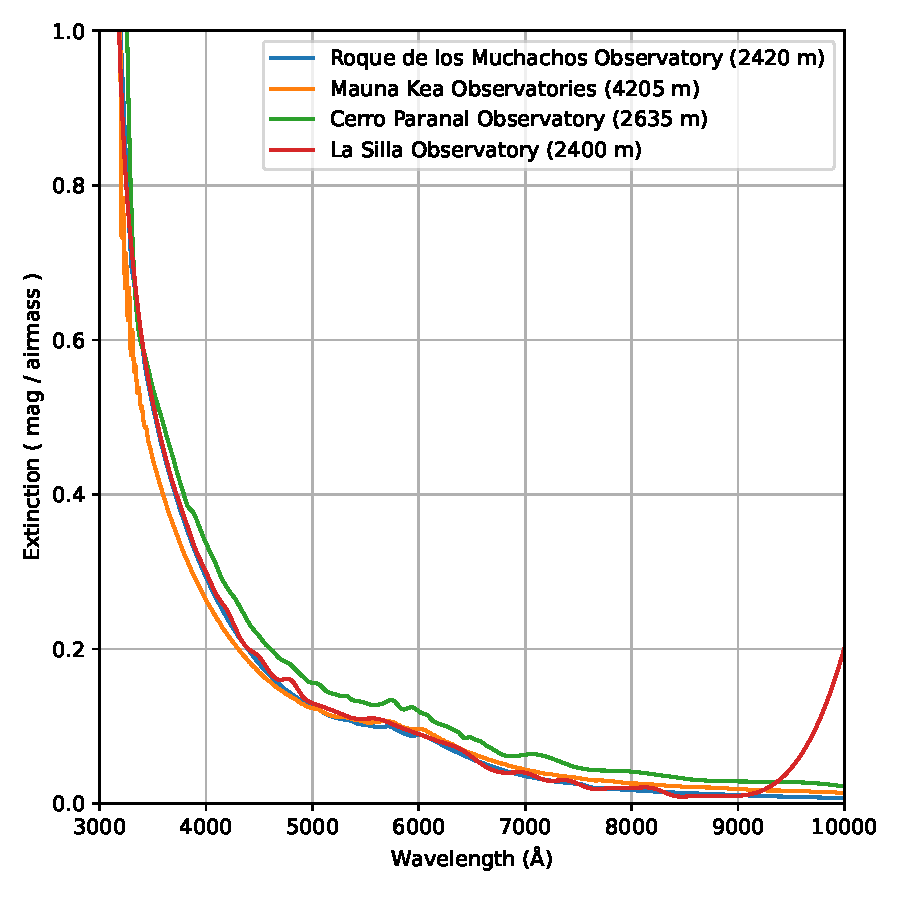
\includegraphics[width=\columnwidth]{fig_07_extinction_curves.pdf}
    \caption{The extinction curves measured at the four sites: Roque de los Muchachos
    Observatory~(2420\,m; blue), Mauna Kea Observatories~(4205\,m; orange),
    Cerro Paranal Observatory~(2635\,m; green), and La Silla Observatory~(2400\,m; red).
    The extinction table of La Silla Observatory terminates at $9000$\,\AA. The rise at
    the red end of the curve is an undesired artefact due to extrapolation using a
    cubic spline. We are explicitly plotting this range to serve as a warning since we
    opt to preserve the input data as provided.}
    \label{fig:extinction}
\end{figure}

\subsection{Telluric Absorption Removal}
During the process of generating the sensitivity function, masks over
the Telluric regions are also used to generate the Telluric absorption
profile from the standard star. The default masking regions are $6850-6960$
and $7580-7700$\ \AA\ only. This profile can then be multiplied
by a factor to be determined in order to remove the Telluric absorption
features in the science target. The best multiplicative factor is found
by minimising the difference between the continuum and the
Telluric-absorption-removed-spectrum. An \textbf{additional} multiplier can
be manually provided to adjust the strength of the subtraction. This is
designed for manually fine-tuning the absorption factor; otherwise, it is
defaulted to $1.0$.

\section{Example Data Reduction Product}
Being a flexible toolkit, \texttt{ASPIRED} is not designed to reduce data for a
specific instrument. Instead, it can be customised to suit many configurations,
as long as they are longslit-like. We demonstrate that with data products
from nine different instruments, most of them have conventional long-slit settings.
In the case of Gemini/GMOS, it has a single spectrum exposed onto three detectors.
LCO/FLOYDS has a beam-splitter to expose the first order red beam and the
second order blue beam into two non-parallel curved spectra on a single chip.
WHT/ISIS demonstrates an extremely low SNR reduction of an ultra-cool white
dwarf with a smooth blackbody-like spectrum. The TNG/DOLORES shows a
simultaneous tracing followed by sequential extraction of three spectra
dispersed in one exposure. We compare the spectra with the published ones if they are available.

\footnote{\url{https://www.wiserep.org/}}

\begin{table*}
    \centering
    \begin{tabular}{l|c|c|c}\hline
        Telescope/Instrument & Object Type                                 & Spectral Resolution & Arc \\\hline\hline
        \multicolumn{4}{c}{Longslit Setup}\\\hline
        SOAR/GHTS            & Type IIn Supernova (AT22NXG)                & ?                   & HgArNe \\
        Liverpool/SPRAT      & Nova shell remnant (DO Aql)                 & ?                   & Xe \\
        GTC/OSIRIS           & BLAP (ZGP-BLAP-09) & ?                   & HgArNe \\
        INT/IDS              & Binary Stars at high resolution             & ?                   & ? \\
        VLT/FORS             & AM CVn                                      & ?                   & ? \\\hline
        \multicolumn{4}{c}{Longslit-like Setup}\\\hline
        Gemini/GMOS          & kilonova (GW170817)                         & ?                   & CuAr \\
        LCO/FLOYDS           & Type II-P (iPTF14hls)                       & ?                   & HgArZn \\\hline
        \multicolumn{4}{c}{Special Use Cases}\\\hline
        TNG/DOLORES          & Common Proper Motion System (dM + dMWD)     & ?                   & ArKrNeHg \\
        WHT/ISIS             & Ultracool White Dwarf                       & 300                 & CuAr \\\hline
\end{tabular}
    \caption{Caption}
    \label{tab:my_label}
\end{table*}



\section{Distribution}
\textsc{ASPIRED} is released under the BSD (3-Clause) License. The
source code is hosted on \textsc{Github}, which can be found at
\url{https://github.com/cylammarco/ASPIRED}. The DOI of each version
can be found at \textsc{zenodo}: \url{https://zenodo.org/record/4463569#.YLjdrKgzYrQ}.
For more straightforward installation, \textsc{ASPIRED} is also available at Python
Package Index~(PyPI): \url{https://pypi.org/project/aspired} so
users can install the software by a simple command of 
\begin{verbatim}
>> pip install aspired.
\end{verbatim}
While the latest stable version can be installed with
\begin{verbatim}
>> pip install git+https://github.com/
    cylammarco/ASPIRED@main
\end{verbatim},
and the latest development version can be installed with 
\begin{verbatim}
>> pip install git+https://github.com/
    cylammarco/ASPIRED@dev-v[X].[Y].X
\end{verbatim}. Where \verb+[X]+ and \verb+[Y]+ are the major and minor version numbers,
\verb+X+ is an actual character of the branch name to denote it as a patch-level maintenance
branch.

It is also possible to clone the entire repository
and install with the setup script with
\begin{verbatim}
>> git clone [url to main/dev/a specific commit]
>> python setup.py
\end{verbatim}
.

\section*{Acknowledgements}
This work was partially supported by OPTICON. This project has
received funding from the European Union's Horizon 2020 research and
innovation programme under grant agreement No 730890. This material
reflects only the authors' views and the Commission is not liable for
any use that may be made of the information contained therein.

This work was partially supported by the Polish NCN grant Daina
No. 2017/27/L/ST9/03221.

MCL is supported by a European Research Council (ERC) grant under the European Union's Horizon 2020 research and innovation program (grant agreement number 852097).

IA is a CIFAR Azrieli Global Scholar in the Gravity and the Extreme Universe Program and acknowledges support from that program, from the ERC under the European Union's Horizon 2020 research and innovation program (grant agreement number 852097), from the Israel Science Foundation (grant number 2752/19), from the United States - Israel Binational Science Foundation (BSF), and from the Israeli Council for Higher Education Alon Fellowship.

The LT is operated on the island of La Palma by Liverpool
John Moores University in the Spanish Observatorio del Roque
de los Muchachos of the Instituto de Astrof{\'i}sica de Canarias with
financial support from the UK Science and Technology Facilities
Council.

This work makes use of observations from the Las Cumbres Observatory
global telescope network. We have made use of the data collected from
the FLOYDS spectrograph on the LCOGT 2m telescope at both Siding Spring,
Australia and Maui, HI, United States.
%%%%%%%%%%%%%%%%% APPENDICES %%%%%%%%%%%%%%%%%%%%%

\appendix

\section{Standard Stars}
\label{appendix:standards}
We provide the list of standard stars available from the ESO, ING and \texttt{iraf} catalogues (see
links in the respective group for the file source). We call the name of the set of
data a \textit{library}; the naming is self-explanatory:

\begin{verbatim}
library_list = [
    `esoctiostan', `esohststan', `esookestan', `esowdstan', `esoxshooter', `ing_oke', `ing_sto',
    `ing_og', `ing_mas', `ing_fg', `irafblackbody', `irafbstdscal', `irafctiocal', 
    `irafctionewcal', `irafiidscal', `irafirscal', `irafoke1990', `irafredcal', `irafspec16cal',
    `irafspec50cal', `irafspechayescal'
]
\end{verbatim}

The following lists all the available stars in each of the libraries.
In \texttt{iraf}, a number of stars with multiple commonly used designations
are run through a name-resolver. We do not provide such utility.
We adopt the name from the filenames as they are.

\subsection{European Southern Observatory~(ESO)}

\subsection*{ESO \citet{1992PASP..104..533H, 1994PASP..106..566H} Standards\footnote{\url{https://www.eso.org/sci/observing/tools/standards/spectra/hamuystandards.html}}}
\begin{verbatim}
esoctiostan = [
    `cd32d9927', `cd_34d241', `eg21', `eg274', `feige110', `feige56', `hilt600', `hr1544',
    `hr3454', `hr4468', `hr4963', `hr5501', `hr718', `hr7596', `hr7950', `hr8634', `hr9087',
    `ltt1020', `ltt1788', `ltt2415', `ltt3218', `ltt3864', `ltt4364', `ltt4816', `ltt6248',
    `ltt7379', `ltt745', `ltt7987', `ltt9239', `ltt9491'
]
\end{verbatim}

\subsection*{ESO \citet{1995AJ....110.1316B, 1996AJ....111.1743B} HST Standards\footnote{\url{https://www.eso.org/sci/observing/tools/standards/spectra/hststandards.html}}}
\begin{verbatim}
esohststan = [
    `agk81d266', `bd28d4211', `bd33d2642', `bd75d325', `bpm16274', `feige110', `feige34',
    `g191b2b', `g93_48', `gd108', `gd50', `grw70d5824', `hd49798', `hd60753', `hd93521',
    `hr153', `hr1996', `hr4554', `hr5191', `hr7001', `hz2', `hz21', `hz4', `hz44', `lb227',
    `lds749b', `ngc7293'
]
\end{verbatim}

\subsection*{ESO \citet{1990AJ.....99.1621O} Standard \footnote{\url{https://www.eso.org/sci/observing/tools/standards/spectra/okestandards_rev.html}}}

\begin{verbatim}
esookestan = [
    `bd25d4655', `bd28d4211', `bd33d2642', `bd75d325', `feige110', `feige34', `feige66',
    `feige67', `g138_31', `g158_100', `g191b2b', `g193_74', `g24_9', `g60_54', `gd108', `gd248',
    `gd50', `grw70d5824', `hd93521', `hz21', `hz4', `hz44', `ltt9491', `ngc7293', `sa95_42'
]
\end{verbatim}

\subsection*{ESO \citet{1995AJ....110.1316B} WD Standards \footnote{\url{https://www.eso.org/sci/observing/tools/standards/spectra/wdstandards.html}}}
\begin{verbatim}
esowdstan = [
    `agk_81d266_005', `alpha_lyr_004', `bd_25d4655_002', `bd_28d4211_005', `bd_33d2642_004',
    `bd_75d325_005', `feige110_005', `feige34_005', `feige66_002', `feige67_002', `g93_48_004',
    `gd108_005', `gd50_004', `gd71', `grw_70d5824_005', `hd93521_005', `hz21_005', `hz2_005',
    `hz44_005', `hz4_004', `lb227_004', `lds749b_005', `ltt9491_002', `ngc7293_005'
]
\end{verbatim}

\subsection*{ESO X-shooter Standards~\citep{2014Msngr.158...16M, 2014A&A...568A...9M}\footnote{\url{https://www.eso.org/sci/observing/tools/standards/spectra/Xshooterspec.html}}}
\begin{verbatim}
esoxshooter = [
    `EG274', `Feige110', `GD153', `GD71', `LTT3218', `LTT7987'
]
\end{verbatim}

\subsection{Issac Newton Group of Telescopes~(ING)}

The ING listing is grouped into five sets by the last name of the authors\footnote{\url{http://www.ing.iac.es/Astronomy/observing/manuals/html_manuals/tech_notes/tn065-100/workflux.html}}.
\subsection*{\citet{1990AJ.....99.1621O} Standards}
\begin{verbatim}
ing_oke = [
    `bd254', `bd28', `bd33', `bd75', `erib', `f110', `f24', `f34', `f66', `f67', `g138', `g158',
    `g191new', `g191old',  `g193', `g24', `g47', `g60', `g99', `gd108', `gd140', `gd190',
    `gd248', `gd50', `grw705new', `grw705old', `grw708', `grw73', `hd935', `he3', `hz14',
    `hz2', `hz21', `hz29', `hz43', `hz44new', `hz44old', `hz4new', `hz4old', `hz7', `l1363',
    `l1512', `l745', `l870', `l930', `l970', `lb1240', `lb227', `lds235', `lds749', `ltt',
    `ngc', `r627', `r640', `sa29', `sa95', `t573', `w1346', `w485'
]
\end{verbatim}

\subsection*{\citet{1977ApJ...218..767S} Standards}

\begin{verbatim}
ing_sto = [
    `bd08', `bd253', `bd28', `bd33', `bd40', `f110', `f15', `f25', `f34', `f56', `f92', `f98',
    `h102', `h600', `hz15', `k27'
]
\end{verbatim}


\subsection*{\citet{1965ApJ...141...83E} Standards}
\begin{verbatim}
ing_og = [`bd17', `bd26', `hd194', `hd849']
\end{verbatim}

\subsection*{\citet{1988ApJ...328..315M} Standards}
\begin{verbatim}
ing_mas = [
    `bd28', `cyg', `eg81', `f110', `f34', `f66', `f67', `g191', `gd140', `h600', `hd192',
    `hd217', `hz14', `hz44', `pg0205', `pg0216', `pg0310', `pg0823', `pg0846', `pg0934',
    `pg0939', `pg1121', `pg1545', `pg1708', `w1346'
]
\end{verbatim}

\subsection*{\citet{1984PASP...96..530F} Standards}
\begin{verbatim}
ing_fg = [`g138', `g158', `g24', `gd248']
\end{verbatim}

\subsection{\texttt{iraf} Standards}
The complete list of \texttt{iraf} standards are available at
\footnote{\url{https://github.com/iraf-community/iraf/tree/main/noao/lib/onedstds}}.

\begin{verbatim}
irafblackbody = [`U', `B', `V', `R', `I', `J', `H', `K', `L', `Lprime', `M']
\end{verbatim}

\begin{verbatim}
irafbstdscal = [
    `hr718', `hr3454', `hr3982', `hr4468', `hr4534', `hr5191', `hr5511', `hr7001', `hr7596',
    `hr7950', `hr8634', `hr9087', `hr15318', `hr74280', `hr100889', `hr188350', `hr198001',
    `hr214923', `hr224926'
]
\end{verbatim}

\begin{verbatim}
irafctiocal = [
    `bd8', `bd25', `bd73632', `cd32', `eg11', `eg21', `eg26', `eg31', `eg54', `eg63', `eg76',
    `eg79', `eg99', `eg139', `eg149', `eg158', `eg248', `eg274', `f15', `f25', `f56', `f98',
    `f110', `feige15', `feige25', `feige56', `feige98', `feige110', `g2631', `g9937', `g16350',
    `h600', `hz2', `hz4', `hz15', `kopf27', `l377', `l1020', `l1788', `l2415', `l2511',
    `l3218', `l3864', `l4364', `l4816', `l6248', `l7379', `l7987', `l8702', `l9239', `l9491',
    `l74546', `l93080', `l97030', `lds235', `lds749', `ltt4099', `ltt8702', `rose627', `w1346',
    `w485a', `wolf1346', `wolf485a'
]
\end{verbatim}

\begin{verbatim}
irafctionewcal = [
    `cd32', `eg21', `eg274', `f56', `f110', `h600', `l377', `l745', `l1020', `l1788', `l2415',
    `l2511', `l3218', `l3864', `l4364', `l4816', `l6248', `l7379', `l7987', `l9239', `l9491',
    `cd32blue', `eg21blue', `eg274blue', `f56blue', `f110blue', `h600blue', `l377blue',
    `l1020blue', `l1788blue', `l2415blue', `l2511blue', `l3218blue', `l3864blue',
    `l4364blue', `l4816blue', `l6248blue', `l7379blue', `l7987blue', `l9239blue',
    `l9491blue', `cd32red', `eg21red', `eg274red', `f56red', `f110red', `h600red', `l377red',
    `l745red', `l1020red', `l1788red', `l2415red', `l2511red', `l3218red', `l3864red',
    `l4364red', `l4816red', `l6248red', `l7379red', `l7987red', `l9239red', `l9491red'
]
\end{verbatim}

\begin{verbatim}
irafiidscal = [
    `40erib', `amcvn', `bd7781', `bd73632', `bd82015', `bd253941', `bd284211', `bd332642',
    `bd404032', `eg11', `eg20', `eg26', `eg28', `eg29', `eg31', `eg33', `eg39', `eg42',
    `eg50', `eg54', `eg63', `eg67', `eg71', `eg76', `eg77', `eg79', `eg91', `eg98', `eg99',
    `eg102', `eg119', `eg129', `eg139', `eg144', `eg145', `eg148', `eg149', `eg158', `eg162',
    `eg182', `eg184', `eg193', `eg247', `eg248', `feige15', `feige24', `feige25', `feige34',
    `feige56', `feige92', `feige98', `feige110', `g88', `g2610', `g2631', `g4718', `g9937',
    `g12627', `g14563', `g16350', `g191b2b', `gd128', `gd140', `gd190', `gh7112', `grw705824',
    `grw708247', `grw738031', `he3', `hz2', `hz4', `hz7', `hz14', `hz15', `hz29', `hz43',
    `hz44', `kopff27', `hiltner102', `hiltner600', `l8702', `l13633', `l14094', `l74546a',
    `l93080', `l97030', `l140349', `l151234b', `lft1655', `lb227', `lb1240', `lds235b',
    `lds749b', `lp414101', `ltt4099', `ltt8702', `ltt13002', `ltt16294', `ross627', `ross640',
    `sa29130', `sao131065', `ton573', `wolf1346', `wolf485a'
]
\end{verbatim}

\begin{verbatim}
irafirscal = [
    `bd082015', `bd174708', `bd253941', `bd262606', `bd284211', `bd332642', `bd404032', `eg50',
    `eg71', `eg139', `eg158', `eg247', `feige15', `feige25', `feige34', `feige56', `feige92',
    `feige98', `feige110', `g191b2b', `hd2857', `hd17520', `hd19445', `hd60778', `hd74721',
    `hd84937', `hd86986', `hd109995', `hd117880', `hd161817', `hd192281', `hd217086', `he3',
    `hiltner102', `hiltner600', `hr7001', `hz44', `kopff27', `wolf1346'
]
\end{verbatim}

\begin{verbatim}
irafoke1990 = [
    `bd75325', `bd284211', `feige34', `feige67', `feige110', `g249', `g13831', `g191b2b',
    `g19374', `gd108', `gd248', `hz21', `ltt9491', `eg71', `eg158', `eg247'
]
\end{verbatim}

\begin{verbatim}
irafredcal = [
    `40erib', `amcvn', `bd7781', `bd73632', `bd174708', `bd262606', `eg20', `eg33', `eg50',
    `eg54', `eg63', `eg67', `eg76', `eg79', `eg91', `eg98', `eg99', `eg102', `eg119', `eg129',
    `eg139', `eg144', `eg145', `eg148', `eg149', `eg158', `eg162', `eg182', `eg184', `eg193',
    `eg247', `eg248', `feige24', `g2610', `g2631', `g4718', `g9937', `g12627', `g14563',
    `g16350', `g191b2b', `gd140', `gd190', `grw705824', `grw708247', `grw738031', `hd19445',
    `hd84937', `he3', `hz29', `hz43', `hz44', `l13633', `l14094', `l151234b', `l74546a',
    `l93080', `l97030', `lds235b', `lds749b', `lft1655', `ltt4099', `ltt8702', `ltt16294',
    `ross627', `ross640', `sa29130', `sao131065', `wolf1346', `wolf485a'
]
\end{verbatim}

\begin{verbatim}
irafspec16cal = [
    `hd15318', `hd30739', `hd74280', `hd100889', `hd114330', `hd129956', `hd188350',
    `hd198001', `hd214923', `hd224926', `hr718', `hr1544', `hr3454', `hr4468', `hr4963',
    `hr5501', `hr7596', `hr7950', `hr8634', `hr9087', `hd15318blue', `hd30739blue',
    `hd74280blue', `hd100889blue', `hd114330blue', `hd129956blue', `hd188350blue',
    `hd198001blue', `hd214923blue', `hd224926blue', `hr718blue', `hr1544blue', `hr3454blue',
    `hr4468blue', `hr4963blue', `hr5501blue', `hr7596blue', `hr7950blue', `hr8634blue',
    `hr9087blue', `hd15318red', `hd30739red', `hd74280red', `hd100889red', `hd114330red',
    `hd129956red', `hd188350red', `hd198001red', `hd214923red', `hd224926red', `hr718red',
    `hr1544red', `hr3454red', `hr4468red', `hr4963red', `hr5501red', `hr7596red', `hr7950red',
    `hr8634red', `hr9087red'
]
\end{verbatim}

\begin{verbatim}
irafspec50cal = [
    `bd284211', `cygob2no9', `eg20', `eg42', `eg71', `eg81', `eg139', `eg158', `eg247',
    `feige34', `feige66', `feige67', `feige110', `g191b2b', `gd140', `hd192281', `hd217086',
    `hilt600', `hz14', `hz44', `pg0205134', `pg0216032', `pg0310149', `pg0823546', `pg0846249',
    `pg0934554', `pg0939262', `pg1121145', `pg1545035', `pg1708602', `wolf1346'
]
\end{verbatim}

\begin{verbatim}
irafspechayescal = [
    `bd284211', `cygob2no9', `eg42', `eg71', `eg81', `eg139', `eg158', `eg247', `feige34',
    `feige66', `feige67', `feige110', `g191b2b', `gd140', `hd192281', `hd217086', `hilt600',
    `hz14', `hz44', `pg0205134', `pg0216032', `pg0310149', `pg0823546', `pg0846249',
    `pg0934554', `pg0939262', `pg1121145', `pg1545035', `pg1708602', `wolf1346'
]
\end{verbatim}


%% For this sample we use BibTeX plus aasjournals.bst to generate the
%% the bibliography. The sample631.bib file was populated from ADS. To
%% get the citations to show in the compiled file do the following:
%%
%% pdflatex sample631.tex
%% bibtext sample631
%% pdflatex sample631.tex
%% pdflatex sample631.tex

\bibliography{main}{}
\bibliographystyle{aasjournal}

%% This command is needed to show the entire author+affiliation list when
%% the collaboration and author truncation commands are used.  It has to
%% go at the end of the manuscript.
%\allauthors

%% Include this line if you are using the \added, \replaced, \deleted
%% commands to see a summary list of all changes at the end of the article.
%\listofchanges

\end{document}

% End of file `sample631.tex'.
